\section{Feature Selection Results}
\subsection{Interpretation of FS results}
In this section the results obtained for each target variable selected are explained in relation to the:
\begin{itemize}
    \item votes received through Borda Count algorithm;
    \item positive or negative correlation assumed in the filter methods;
\end{itemize}
Similarity between the 2 test sets are visible for many factors that influence both particulate matter and ammonia.
For instance, DTM average elevation and slope ('h\_mean' and 'slope\_mean' respectively) received many votes in both cases, since air pollution affect more urban than mountain areas.
The results show also how particulate matter and ammonia are influenced by meteorological parameters.
Air temperature ('temp\_2m') increases with global radiation ('rad\_glob\_int'), while pollutants significantly decreased\cite{li2015particulate}. \\
Also the pressure contribute to them ('press' with a remarkable number of votes between 100 and 125), since causes stable atmospheric condition that make PM harder to be disseminated. 
Instead, pollutants are negatively correlated to wind speed ('e\_wind'), since their concentration tends to turn down with it. Wind is a marker for the horizontal transport of air pollutants.\\
It can be observed also the negative correlation between pollution and air humidity ('air\_hum\_int').
Under increased humidity conditions, PM and ammonia may be prone to a washout mechanism due to moisture in the air, causing a particulate reduction\cite{biglari2017relationship}.\\
Another pollutant with a significant number of votes is the aerosol optical depth ('aod\_047' and 'aod\_055'). It's evident that AOD has a strong correlation with pollutants, due to the fact that they are suspension of a solid or liquid particles in the air. AOD in fact measure the atmospheric aerosols.
\begin{figure}[H]
    \centering
    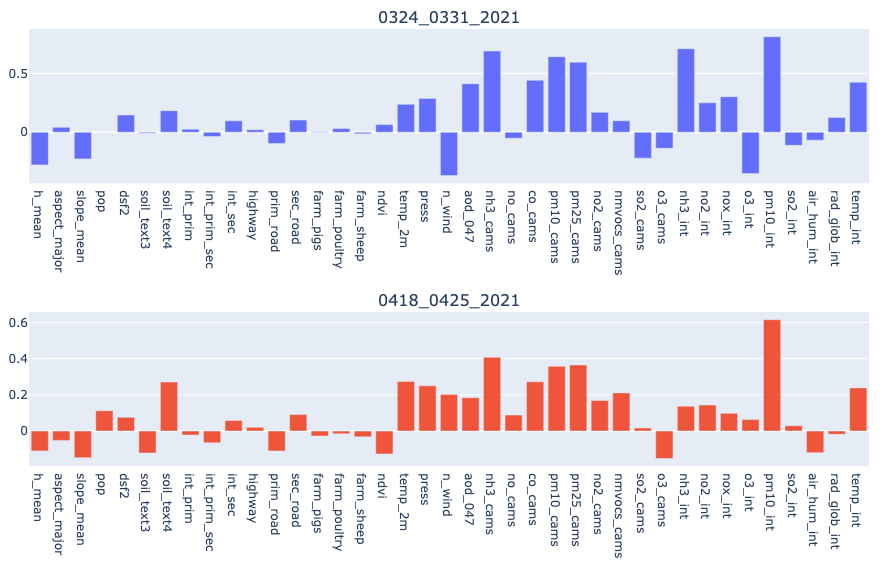
\includegraphics[scale=0.45]{src/images/tests/correlations_pm25.png}
    \caption{Correlation of Pearson index for the period between 24th-21st March and 18th-25th April having PM2.5 as target variable.}
    \label{fig:overview}
\end{figure}

\subsection{PM25 as target variable}
Fine particulate matter (PM2.5) is one of the most common air pollutant in our environment. 
It primarily comes from transport vehicle (such as car, truck and bus), industry, burning of fuels and household activities.\\ \par
During the 5 periods, it's shown that PM25, as the other pollutants, change over the time. Air pollution change accordingly to the type of climate and atmospheric conditions.\\
\begin{comment}
In the tests is also visible the score obtained by ozone ('o3\_int') which tends to be positively correlated in the period between 18 and 25 April.\\
This, as mentioned before, is possibly due to their common precursors, such as nitrogen oxides and volatile organic compounds and their simultaneous generation in photochemical reactions. \\
\end{comment}
Air pollution analysis can confirm the presence of high quantity in winter and heating season and low in summer months\cite{cichowicz2017dispersion}. This is not applied to the ozone ('o3\_int' and 'o3\_cams'), which should be, on the contrary, higher during summer due to combination of heat and sunlight which reacts with nitrogen oxides (NOx) and volatile organic compounds. Indeed, for the week between 17 and 24 July a negative correlation between them is found, due to the fact that is inversely related to PM25.\\
By the bar plots attached in the figure \ref{fig:fs_pm25}, the most correlated variables to PM25 belong mostly to pollutant. In particular PM10 provided by ARPA and CAMS, in the various test executed is one of the most correlated pollutant. Indeed, 'pm10\_int' and 'pm10\_cams' have always a number votes more than 120. Strong positive correlation between PM25 and PM10 is also proved in literature\cite{zhou2016concentrations}. 
It's visible a correlation with nitrogen dioxide('no2\_int'), a strong greenhouse gas which is related, as particulate matter, to biomass burning, industrial processes, households and road transport\cite{zellner2000john}\cite{maranzano2022air}.
From nitrogen dioxide derives also the chemical relation with the other nitrogen oxides ('nox\_int'), such as nitrogen monoxide ('no\_int').
\\
Observing the results regarding intense agriculture, it's evident that ammonia ('nh3\_int' and 'nh3\_cams') received as PM10 most votes of all in spring period due to its strong positively correlation. 
We can assume that the main emission source of ammonia is the intense agriculture, since was responsible for the 92\% of the total by EEA country members in 2017\cite{maranzano2022air}.\\
Indeed, during this periods, application of fertilizer contribute to ammonia and particulate matter composition.
Significantly more fertilizer is applied in the spring than summer and winter season due to crop cycles\cite{goebes2003ammonia}.
So we can assume that intense agriculture is one of the factor that influence the pm25 formation, but only in a certain period of the year.\\
\pagebreak
\clearpage
\begin{figure}[H]
\centering
\subfloat[10 Km resolution with mountains]{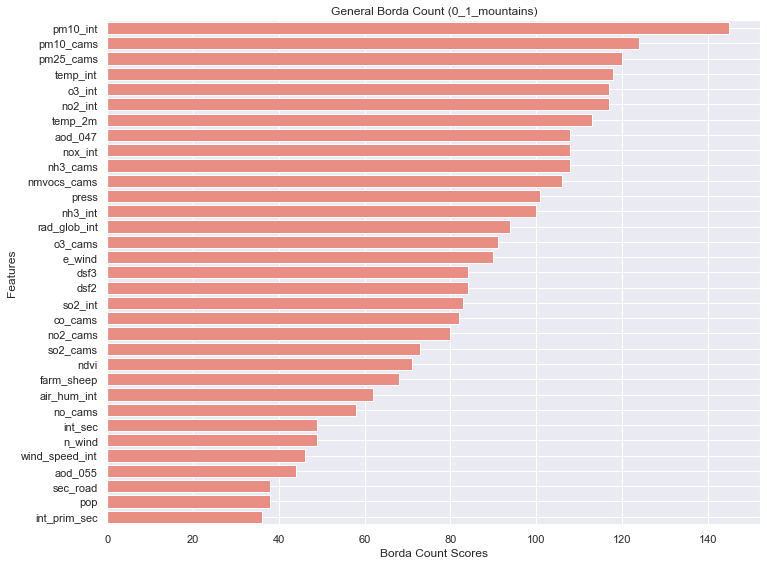
\includegraphics[scale =0.42]{images/tests/0_1_mountainspm25_st.png}}\\
\subfloat[1 Km resolution without mountains]{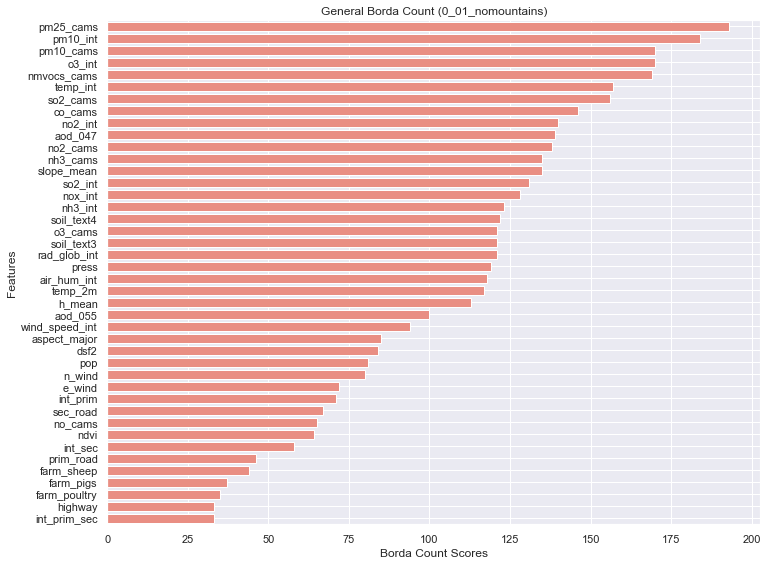
\includegraphics[scale =0.42]{images/tests/0_01_nomountainspm25_st.png}}
\caption{FS results obtained with PM2.5 as target variable.}
\label{fig:fs_pm25}
\end{figure}
\subsection{NH3 as target variable}
Ammonia (NH3) is a reactive and soluble alkaline gas. It's one of the main sources of nitrogen pollution and come from both natural and anthropogenic sources, such as agriculture.
The process of ammonia evaporation commonly takes place when nitrogen is originated by urea of animal livestock, and fertilize. \\
In the results obtained along the 5 period, stands out the ammonia provided by CAMS model ('nh3\_cams') which, due to the fact that represents the same pollutant, is strongly correlated. Variables related to atmospheric condition are weighted with scores of the same order of magnitude of the previous test set, since ammonia is dispersed in the environment as particulate matter and other pollutants.\\
We can observe in figure \ref{fig:fs_nh3} also variable related to pm10 and pm25('pm10\_int', 'pm10\_cams','pm25\_int' and 'pm25\_cams'), because ammonia contribute for the formation of secondary particulate matter (pm25 in particular\cite{zhu2015sources} .\\
Correlation of ammonia with respect to intensive agricultural is also feasible by the high positive correlation with agricultural areas (modelled by 'dsf2' variable) and the Normalized Difference Vegetation Index ('ndvi').\\
Other important weighted features are the ones related to intense farming ('farm\_sheeps', 'farm\_pigs', 'farm\_poultry' and 'farms') which are responsible for ammonia and methane release ('ch4\_s5p' has a meaningful positive correlation with respect to NH3).\\
Indeed, animal urine and faeces imply the release of respectively ammonia and methane in the atmosphere\cite{saggar2004review}.\\
It can be viewed also how road infrastructure variables contribute to ammonia. In particular the correlation between them is negative, since ammonia emission from agriculture occurs usually far from urban and traffic areas.\\
So we can suggest that ammonia in Lombardy should be very related to the use of fertilizer in agriculture areas and animal livestock in farms.
\bigbreak
So overall, the results obtained in the feature selection demonstrate two things.  
First, fine particulate should be very correlated to ammonia in the planting period (spring) . Second, ammonia is stricly related to agriculture and farming activity, in line with previous studies.
\pagebreak
\clearpage
\begin{figure}[H]
\centering
\subfloat[10 Km resolution with mountains]{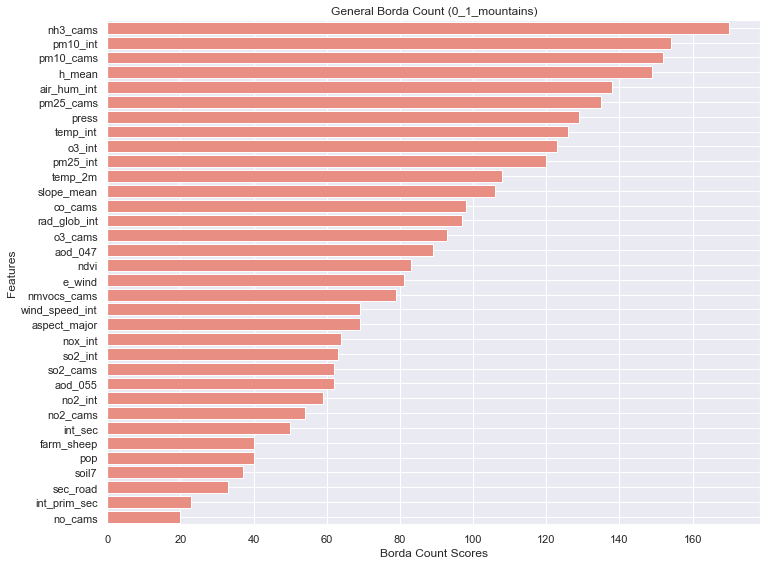
\includegraphics[scale =0.42]{images/tests/0_1_mountainsnh3_st.png}}\\
\subfloat[1 Km resolution without mountains]{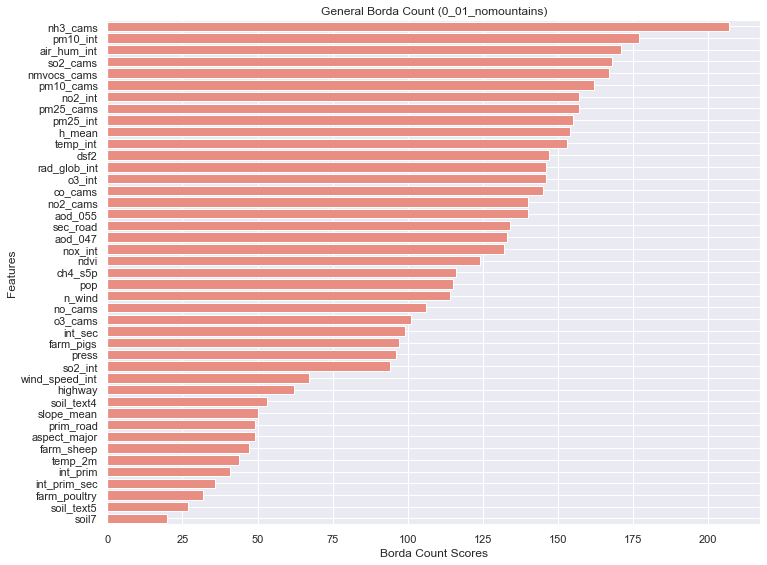
\includegraphics[scale =0.42]{images/tests/0_01_nomountainsnh3_st.png}}
\caption{FS results obtained with Ammonia (NH3) as target variable.}
\label{fig:fs_nh3}
\end{figure}
\section{Data Modelling Results}
\subsection{Interpretation of validation results with ARPA sensor}
Models assure a consistent accuracy.
Errors obtained in the results by the validation through Particulate Matter decrease in function of the higher resolution.
Higher resolution, as a matter of fact, implies a larger number of sample for training and so a better accuracy as consequence.
Instead, in the models for ammonia estimation there are no relevant differences between the 2 resolutions.
With PM25 as target variable at 10 km resolution there is a lower statistical accuracy than at 1km, with MAE respectively around 1 and 0.5 ug/m\textsuperscript{3}(Table \ref{tab:res1km}). 
\begin{table}[H]
\begin{tabular}{rrrrrr}
\hline
      &   24/03-31/03 &   18/04-25/04 &   17/07-24/07 &   3/09-10/09 &   7/10-14/10 \\
\hline
  MAE\_sensor   &            2.114 &            1.329 &            0.825 &            1.311 &            0.752 \\
  MSE\_sensor   &            8.825 &            3.047 &            1.19  &            3.016 &            0.917 \\
  R2\_sensor    &            0.712 &            0.61  &            0.504 &            0.716 &            0.846 \\
\hline
\end{tabular}
\caption{Random Forest prediction for PM2.5 at 10 km, excluding zones with mountains.}
\end{table}
\begin{table}[H]
\begin{tabular}{rrrrrr}
\hline
     &   24/03-31/03 &   18/04-25/04 &   17/07-24/07 &   3/09-10/09 &   7/10-14/10 \\
\hline
   MAE\_sensor   &            0.465 &            0.36  &            0.33  &            0.325 &            0.269 \\
  MSE\_sensor   &            0.654 &            0.333 &            0.266 &            0.291 &            0.174 \\
   R2\_sensor    &            0.983 &            0.962 &            0.926 &            0.98  &            0.979 \\
\hline
\end{tabular}
\caption{Random Forest prediction for PM2.5 at 1 km, including zones with mountains.}
\label{tab:res1km}
\end{table}

\begin{table}[H]
\begin{tabular}{rrrrrr}
\hline
     &   24/03-31/03 &   18/04-25/04 &   17/07-24/07 &   3/09-10/09 &   7/10-14/10 \\
\hline
  MAE\_sensor   &            1.293 &            0.238 &            2.25  &            2.304 &            1.504 \\
  MSE\_sensor   &           11.206 &            0.149 &           20.907 &           24.379 &           16.739 \\
  R2\_sensor    &            0.972 &            0.997 &            0.927 &            0.943 &            0.917 \\
\hline
\end{tabular}
\caption{Random Forest prediction for NH3 at 1 km, excluding zones with mountains.}
\label{tab:nh3}
\end{table}
In the model for ammonia estimation instead, this error is around 2 with MSE always higher than 20 (Table \ref{tab:nh3}).
This difference should be given by different number of ground sensor for each pollutant. The sample of particulate matter measurement in fact is larger than the ammonia's one (figure \ref{fig:comparison-sensors}).
\begin{figure}[H] 
    \centering
    \subfloat[PM25 as target variable]{%
        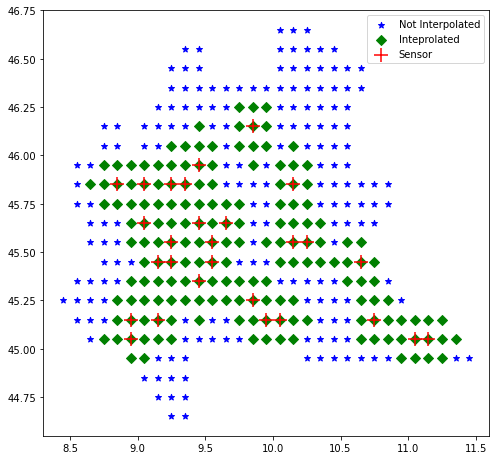
\includegraphics[width=0.5\textwidth]{src/images/pm25_sensors.png}%
        %
        }%
    \hfill%
    \subfloat[NH3 as target variable.]{%
        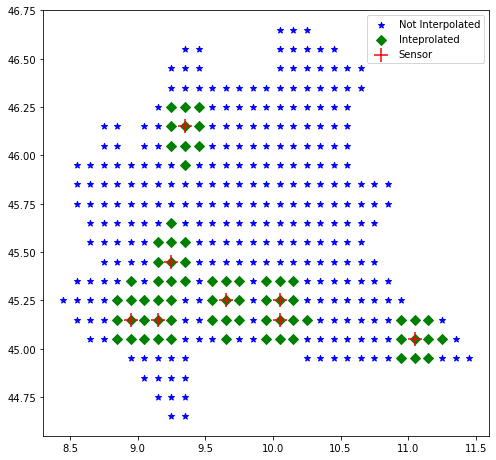
\includegraphics[width=0.5\textwidth]{src/images/nh3_sensors.png}%
        %
        }%
    \caption{In these images are shown the observations at 10km resolution of each different target variable used in this case of study. The legend shows whether the cell has an interpolated value with KNN or not. In addition ground sensor from which interpolation is performed are added}
    \label{fig:comparison-sensors}
\end{figure}

We can observe that generally Random Forest model makes more accurate predictions than the Neural Network by Keras. This may caused by the fact that RF algorithm uses ensemble learning method for regression, a technique that joins estimation from multiple models for having more accurate predictions than a single model. 
R\textsuperscript{2} in each test assumes a positive value (around 50\% for Neural Network and around 80\% for RF), meaning that the pollutants take in consideration in this case of study can be explained by the regression models. 
\subsection{Comparison with CAMS model}
The comparison between models of my results and CAMS data shows how values are very far from them. MAE for pm25 values is around 5 while for ammonia around 10 ug/m\textsuperscript{3}. Values assumed by MSE, since the distance between the results is squared, exceed 40 for PM25 and 170 for NH3 in each different configurations.
Another proof of difference between the 2 models is the R\textsuperscript{2} value which is assumes a negative value in most of the cases. It proves the presence of a big difference between training and test values. 

\begin{table}[H]
\begin{tabular}{rrrrrr}
\hline
     &   24/03-31/03 &   18/04-25/04 &   17/07-24/07 &   3/09-10/09 &   7/10-14/10 \\
\hline
   MAE\_cams     &            8.966 &            7.566 &            1.936 &            3.574 &            3.974 \\
  MSE\_cams     &          106.414 &           71.818 &            6.213 &           16.81  &           20.988 \\
   R2\_cams      &           -1.821 &           -7.099 &           -0.727 &           -0.18  &           -1.578 \\
\hline
\end{tabular}
\caption{Random Forest prediction for PM2.5 at 1 km, including zones with mountains.}
\end{table}
\begin{table}[H]
\begin{tabular}{rrrrrr}
\hline
     &   24/03-31/03 &   18/04-25/04 &   17/07-24/07 &   3/09-10/09 &   7/10-14/10 \\
\hline
  MAE\_cams     &           18.401 &           10.414 &           11.746 &           14.18  &           12.012 \\
  MSE\_cams     &          368.858 &          147.652 &          323.418 &          456.145 &          188.65  \\
  R2\_cams      &            0.136 &           -1.511 &           -0.158 &           -0.001 &           -0.06  \\
\hline
\end{tabular}
\caption{Random Forest prediction for NH3 at 1 km, excluding zones with mountains.}
\end{table}
Obviously the model of Copernicus Atmosphere Monitoring Service provide different results by one obtained by me, since is build very differently. CAMS is built through ensemble median, averaged by eleven European air quality forecasting systems. Therefore, median model should perform better than the individual model products\cite{riccio2007seeking}; 
Anyway, through information collected on the Copernicus website, only a limited number of ground observation are detected in the Italy territory. As it can be seen by figure TODO in Italy there's only 1 observation in Sardinia for PM25 detection. Nothing was found for Ammonia.
So, by the larger number of ground observation provided by ARPA in this data collection this model should perform better in this local scale.
\bigbreak
Based on these results, we can point that Random Forest is more precise than Neural Network model and that the performance are higher for particulate matter than ammonia estimation.
Random Forest indeed is one the most preferred also in literature prediction model for its easy configuration. (CITE TODO)
\subsection{Importance of the FS}
Feature selection is meaningful for the pre processing phase, since aims to discard eventually useless variable and to take only the ones really relevant to the target variable. In the results obtained we can detected that selection of variable with FS assume a key role for sample of small size. 
Indeed, in the tests with resolution 10 Km model there's a feasible difference between the data trained by variable from FS and the ones chosen randomly. 
This gap become negligible with higher resolution, because ML algorithms accuracy increase with sample size(CITATION).
\begin{tabular}{rrrrrr}
\hline
          &   24/03-31/03 &   18/04-25/04 &   17/07-24/07 &   3/09-10/09 &   7/10-14/10 \\
\hline
   MAE\_sensor &         2.061 &         1.604 &         0.885 &        1.601 &        1.2   \\
    MSE\_sensor &         6.531 &         4.303 &         1.311 &        4.497 &        2.457 \\
    R2\_sensor  &         0.767 &         0.328 &         0.298 &        0.58  &        0.683 \\
    MAE\_cams   &         7.8   &         6.554 &         2.113 &        3.06  &        3.478 \\
    MSE\_cams   &        86.279 &        57.562 &         7.565 &       13.266 &       16.591 \\
    R2\_cams    &        -2.147 &        -8.102 &        -3.386 &       -0.239 &       -1.158 \\
\hline
\end{tabular}
\begin{comment}
ps://www.sciencedirect.com/topics/agricultural-and-biological-sciences/agricultural-pollution 
https://pure.iiasa.ac.at/id/eprint/14769/1/Reduction%20of%20NH3%20emissions%20from%20agriculture%20in%20the%20Hai%20River%20Basin%20in%20China.pdf

https://towardsdatascience.com/batch-mini-batch-stochastic-gradient-descent-7a62ecba642a
\end{comment}
